%
%Introduction
%


\section{Motivation}
\subsection{Git}

 Git\cite{git} is a famous distributed revision control and source code
management system with an emphasis on speed.


One of it's main features is its fast branching and merging. That is because branches in git are very lightweight, a branch in git is only a reference to a single commit.


It has complete history and full revision tracking capabilities;


Its commands are divided into two types:
\begin{itemize}
\item Porcelain commands: The type of commands that the normal user should be using most of the time, very high-level;
\item Plumbling commands: The low-level commands, commonly used for some tweaks.
\end{itemize}

But git is not a perfect world, as we can see by some random internet quotes:

\begin{quote}
``What a pity that it’s so hard to learn, has such an unpleasant command line interface, and treats its users with such utter contempt."
\end{quote}
\begin{flushright}
\textit{\href{http://steveko.wordpress.com/2012/02/24/10-things-i-hate-about-git/}{10 things I hate about Git}}
\end{flushright}

\begin{quote}
``The man pages are one almighty “f*ck you”. They describe the commands from the perspective of a computer scientist, not a user."
\end{quote}
\begin{flushright}
\textit{\href{http://steveko.wordpress.com/2012/02/24/10-things-i-hate-about-git/}{10 things I hate about Git}}

\end{flushright}

\begin{quote}
``(...) there are lots of "cheat sheets" floating around about how to use git tools - I think this is evidence that [...] many
 people have to write "GIT for mortals" pages..."
\end{quote}
\begin{flushright}
\textit{Perl Mailing List}
\end{flushright}


Git is a complex tool, it is not simple to use and its manual is obscure.
Its commands are multi-purpose and sometimes they won't work as you expect them to, or even do something that isn't even mentioned on the manual.


For those reasons, we purpose the creation of a formal git model to alleviate some of these problems.
With an actual git model it would be easier to predict the system behaviour, as well as verify some of the system's properties.
A model would also help with the finding of bugs, because you could say that an operations didn't run as expected by the formal model.
The main problem would be how accurate the model would be. It needs to be validated!


But validating a formal model of an existing system is not a easy task. Deriving the model from the code is a option, just as well as trial and error, our approach is test case generation.

\section{Solution}


Model validation through test case generation is an approach where we use a model to generate test runs with the input of a modelled operation and its expected result, which is then compared with a run of the actual system operation for the same input, if they do not match then the model is not accurate or the system is bugged.

\begin{figure}[H]
\centering
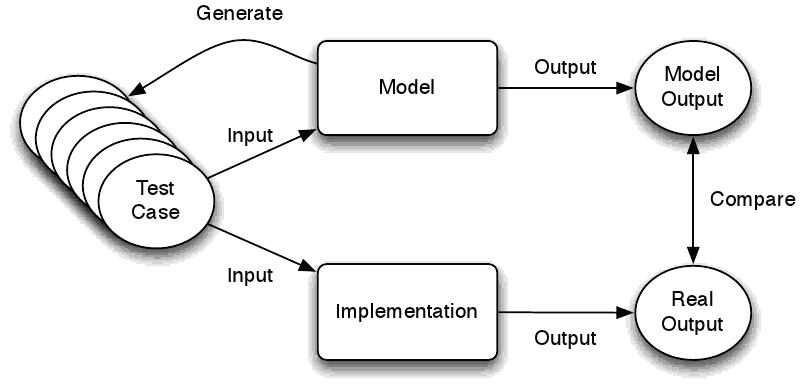
\includegraphics[width=\textwidth]{images/test-case.png}
\caption{Model validation through test case generation}
\end{figure}


We are using a Alloy\cite{alloy} model to represent git, because Alloy provides us the features needed for the use of model validation through test case generation, we can use predicates model the operations and make use of its solving to generate the test cases. It also has a Java API which we used to automate the process.


This approach makes the validation highly automatic, but we must have caution about our pre-conditions strength. Pre-conditions too strong won't fully test the operation and it is hard to recognize when a pre-condition is too strong, so we might miss some bugs.



